\section{Teaching with reduced models and native Pyomo.DoE}
\label{sec:teaching-doe}
This supplement adds the teaching comparison and native Pyomo.DoE demonstration
completed after the overnight study. Its four designs use a separate,
single-model protocol from the ensemble designs in the main results. The saved
fits, uncertainty calculations and literature claims in the preceding sections
are unchanged.

\subsection{One stage is sufficient for the core teaching exercise}
Use $n=1$ to teach parameter estimation, local information and input design.
It has two dynamic states and three unknown transfer parameters, $K$, $\tau$
and $\theta$. It retains the original four-parameter model's response under the
studied observation equation and startup conditions while removing a redundant
parameter direction. Add $n=2$ as an extension on delay shape, model comparison
and numerical discretization. It has three states and still three unknown
parameters. The available fits do not require higher orders for this exercise.

The independently optimized joint $n=1$ and original fits differ in predicted
temperature by less than $1.5\times10^{-7}\,{}^\circ\mathrm C$ on calibration
and held-out records. Parameter reduction therefore preserves these predictions.
Table~\ref{tab:teaching-prediction} gives the cold-start comparison on the joint
calibration and eleven duplicate-excluded held-out files, without refitting
to those files. The $n=2$ joint calibration RMSE is about $12.5\%$ higher and
its pooled held-out RMSE about $0.06\%$ higher. On the step-only calibration,
$n=2$ lowers RMSE from $0.1573$ to $0.1529\,{}^\circ\mathrm C$, about $2.8\%$.
Initialization can reverse the order ranking. These results do not establish a
general predictive advantage for an additional delay stage.
% Generated by teaching_followup/render_report_tables.py
\begin{table}[htbp]
\centering
\small
\caption{Cold-start joint fits and pooled held-out prediction error. RMSE is in degrees Celsius.}
\label{tab:teaching-prediction}
\begin{tabular}{lrr}
\toprule
Model & Calibration RMSE & Held-out RMSE \\
\midrule
Original four-parameter & 0.4115 & 3.3588 \\
$n=1$ & 0.4115 & 3.3588 \\
$n=2$ & 0.4630 & 3.3608 \\
\bottomrule
\end{tabular}
\end{table}


The $n=1$ pole labels can be exchanged globally. A convention such as
$\tau\geq\theta$ chooses the short-delay representative; a full-rank local
information matrix does not detect the other mode. The $n=2$ repeated delay pole
distinguishes it from a distinct thermal pole, while coincident poles remain
nonregular. Neither reduced formulation identifies a unique member of the
original physical parameter family.

\subsection{Residual correlation changes uncertainty more than model order}
Table~\ref{tab:teaching-blocks} compares nominal $95\%$ percentile intervals
from $400$ refits per method using the same centered empirical residual pool.
Changing independent resampling to $60$-sample circular blocks widens the delay
interval by factors of $6.66$ for $n=1$ and $6.23$ for $n=2$. Sixty samples
are roughly one minute in these records. This isolates retained dependence
from the change of marginal error scale that occurs when comparing empirical
resampling with fixed-scale Gaussian simulation.
% Generated by teaching_followup/render_report_tables.py
\begin{table}[htbp]
\centering
\small
\caption{Delay percentile intervals (s) from the same centered residual pool; 400 refits per method. Width ratio compares 60-sample blocks with independent resampling.}
\label{tab:teaching-blocks}
\begin{tabular}{lrrr}
\toprule
Model & Independent & 60-sample blocks & Width ratio \\
\midrule
$n=1$ & [16.41, 16.70] & [15.62, 17.56] & 6.66 \\
$n=2$ & [15.22, 15.56] & [14.31, 16.44] & 6.23 \\
\bottomrule
\end{tabular}
\end{table}


These are conditional intervals: centering removes the record-specific mean
error, block length is an assumption, and the $n=1$ interval excludes its global
swapped-pole mode. The controlled OU60 simulation provides a separate coverage
check. With the thermal mean correct by construction, nominal $95\%$
IID fitted-variance delay intervals cover only $66/300$ datasets for $n=1$
and $56/300$ for $n=2$. HAC60 raises these counts to $235/300$ and $249/300$.
The real-data one-component OU fits retain innovation lag-one correlations near
$-0.5$. Neither the wider bootstrap intervals nor the OU likelihood establishes
an adequate real-data discrepancy model.

\subsection{A three-parameter Pyomo.DoE implementation}
The demonstration uses Pyomo $6.10.0$ and a Parmest \texttt{Experiment} subclass
with the experiment-input, experiment-output, measurement-error and
unknown-parameter suffixes. The implementation follows the
\href{https://pyomo.readthedocs.io/en/stable/explanation/analysis/doe/guide.html}{official Pyomo.DoE quick-start guide}
(accessed October 21, 2026). Each reduced model yields a full-rank $3\times3$
local information matrix. Under the original four-parameter single-output
formulation, the exact four-dimensional determinant vanishes because the rank
is three. Finite-difference roundoff cannot restore the missing information.

Let $p=(K,\tau,\theta)$, $\eta=\log p$ and
$J_{ij}=\partial\mu(t_i)/\partial\eta_j$. Relative-parameter scaling in
Pyomo.DoE supplies this local log-parameter sensitivity. The design maximizes
the log determinant of
\begin{equation}
 F_\eta=J^\mathsf{T}\Sigma^{-1}J.
\end{equation}
There is no prior information matrix. The nominal parameters are the saved joint
cold fits. Each of the four model/covariance cases uses two optimization starts,
constant $50\%$ and alternating $30/70\%$ command. The selected local result
has the larger converged objective; no global optimality claim follows.

The experiment lasts $900$ s and observes temperature every $10$ s, excluding
the initial value, for $90$ observations. Seven command knots are spaced
$150$ s apart, with linear interpolation. Commands lie between $0$ and $100\%$,
adjacent knots differ by at most $60$ percentage points, and integrated command
is at most $45000$ percent-seconds. The ambient and initial temperature are
$22.2\,{}^\circ\mathrm C$, with cold delay states. Nominal collocation
temperatures are constrained below $84.99\,{}^\circ\mathrm C$, retaining a
$0.01\,{}^\circ\mathrm C$ guard below the independent $85\,{}^\circ\mathrm C$
acceptance limit.

The measurement-error suffix contains standard deviations. Its built-in
weighting assumes independent errors. For the correlated comparator, the
stationary OU law has known marginal standard deviation
$\sigma=0.25\,{}^\circ\mathrm C$ and known correlation length $60$ s.
With $\phi_i=\exp[-(t_i-t_{i-1})/60]$, transformed mean outputs are
\begin{equation}
 \widetilde\mu_1=\mu_1,\qquad
 \widetilde\mu_i=\frac{\mu_i-\phi_i\mu_{i-1}}{\sqrt{1-\phi_i^2}},
 \quad i\geq2.
\end{equation}
Applying independent weighting with standard deviation $\sigma$ to these
outputs gives the full-covariance information matrix above. Covariance
parameters are held fixed throughout.

\subsection{The selected inputs heat, cool and heat again}
Table~\ref{tab:teaching-doe} compares each selected input with constant $50\%$
under the same model and working covariance. The D-information multiplier is
$[\det(F_{\mathrm{selected}})/\det(F_{\mathrm{constant}})]^{1/3}$.
It ranges from $3.67$ to $4.12$. The local delay SD falls from
$0.728$ to $0.272$ s for $n=1$ under independent errors and from
$1.627$ to $0.678$ s under known OU60 errors. The corresponding $n=2$ values
are $0.630$ to $0.245$ s and $1.225$ to $0.536$ s.
% Generated by teaching_followup/render_report_tables.py
\begin{table}[htbp]
\centering
\small
\caption{Conditional local delay standard deviations (s) and D-information multipliers for the selected and constant-input designs. Each row uses its own working covariance and a hypothetical marginal error SD of $0.25\,{}^\circ\mathrm C$.}
\label{tab:teaching-doe}
\begin{tabular}{llrrr}
\toprule
Model & Error law & Constant SD & Selected SD & D multiplier \\
\midrule
$n=1$ & IID & 0.728 & 0.272 & 4.12 \\
$n=2$ & IID & 0.630 & 0.245 & 4.09 \\
$n=1$ & Known OU60 & 1.627 & 0.678 & 3.80 \\
$n=2$ & Known OU60 & 1.225 & 0.536 & 3.67 \\
\bottomrule
\end{tabular}
\end{table}


These SDs concern hypothetical future measurements at the fixed fitted
parameters and error law. They are separate from the empirical residual
intervals above. The information gains do not measure a realized improvement
in prediction accuracy.

Figure~\ref{fig:teaching-experiments} shows the selected commands and their
nominal temperature responses. All four inputs start at $100\%$ for $2.5$ min,
ramp down through about $86\%$ at $5$ min and $26$--$34\%$ at $7.5$ min,
and reach zero at $10$ min. They remain mostly off until $12.5$ min, then ramp
to $60$--$66\%$ at $15$ min. Each uses the same integrated command as the
constant $50\%$ reference, concentrating heat early to create heating and
cooling transients. Table~\ref{tab:teaching-commands} supplies the knot values.

The predicted peak is about $84.93\,{}^\circ\mathrm C$ at $5.4$--$5.5$ min.
Changing the working covariance has a modest effect on the $n=1$ schedule.
For $n=2$, the two selected commands differ by less than
$5\times10^{-7}$ percentage points. Thus nearly identical input schedules can
coexist with substantially different uncertainty calculations. The correlated
assumption gives selected-input delay SDs about $2.2$--$2.5$ times their
independent-error counterparts in this comparison.

\begin{figure}[p]
 \centering
 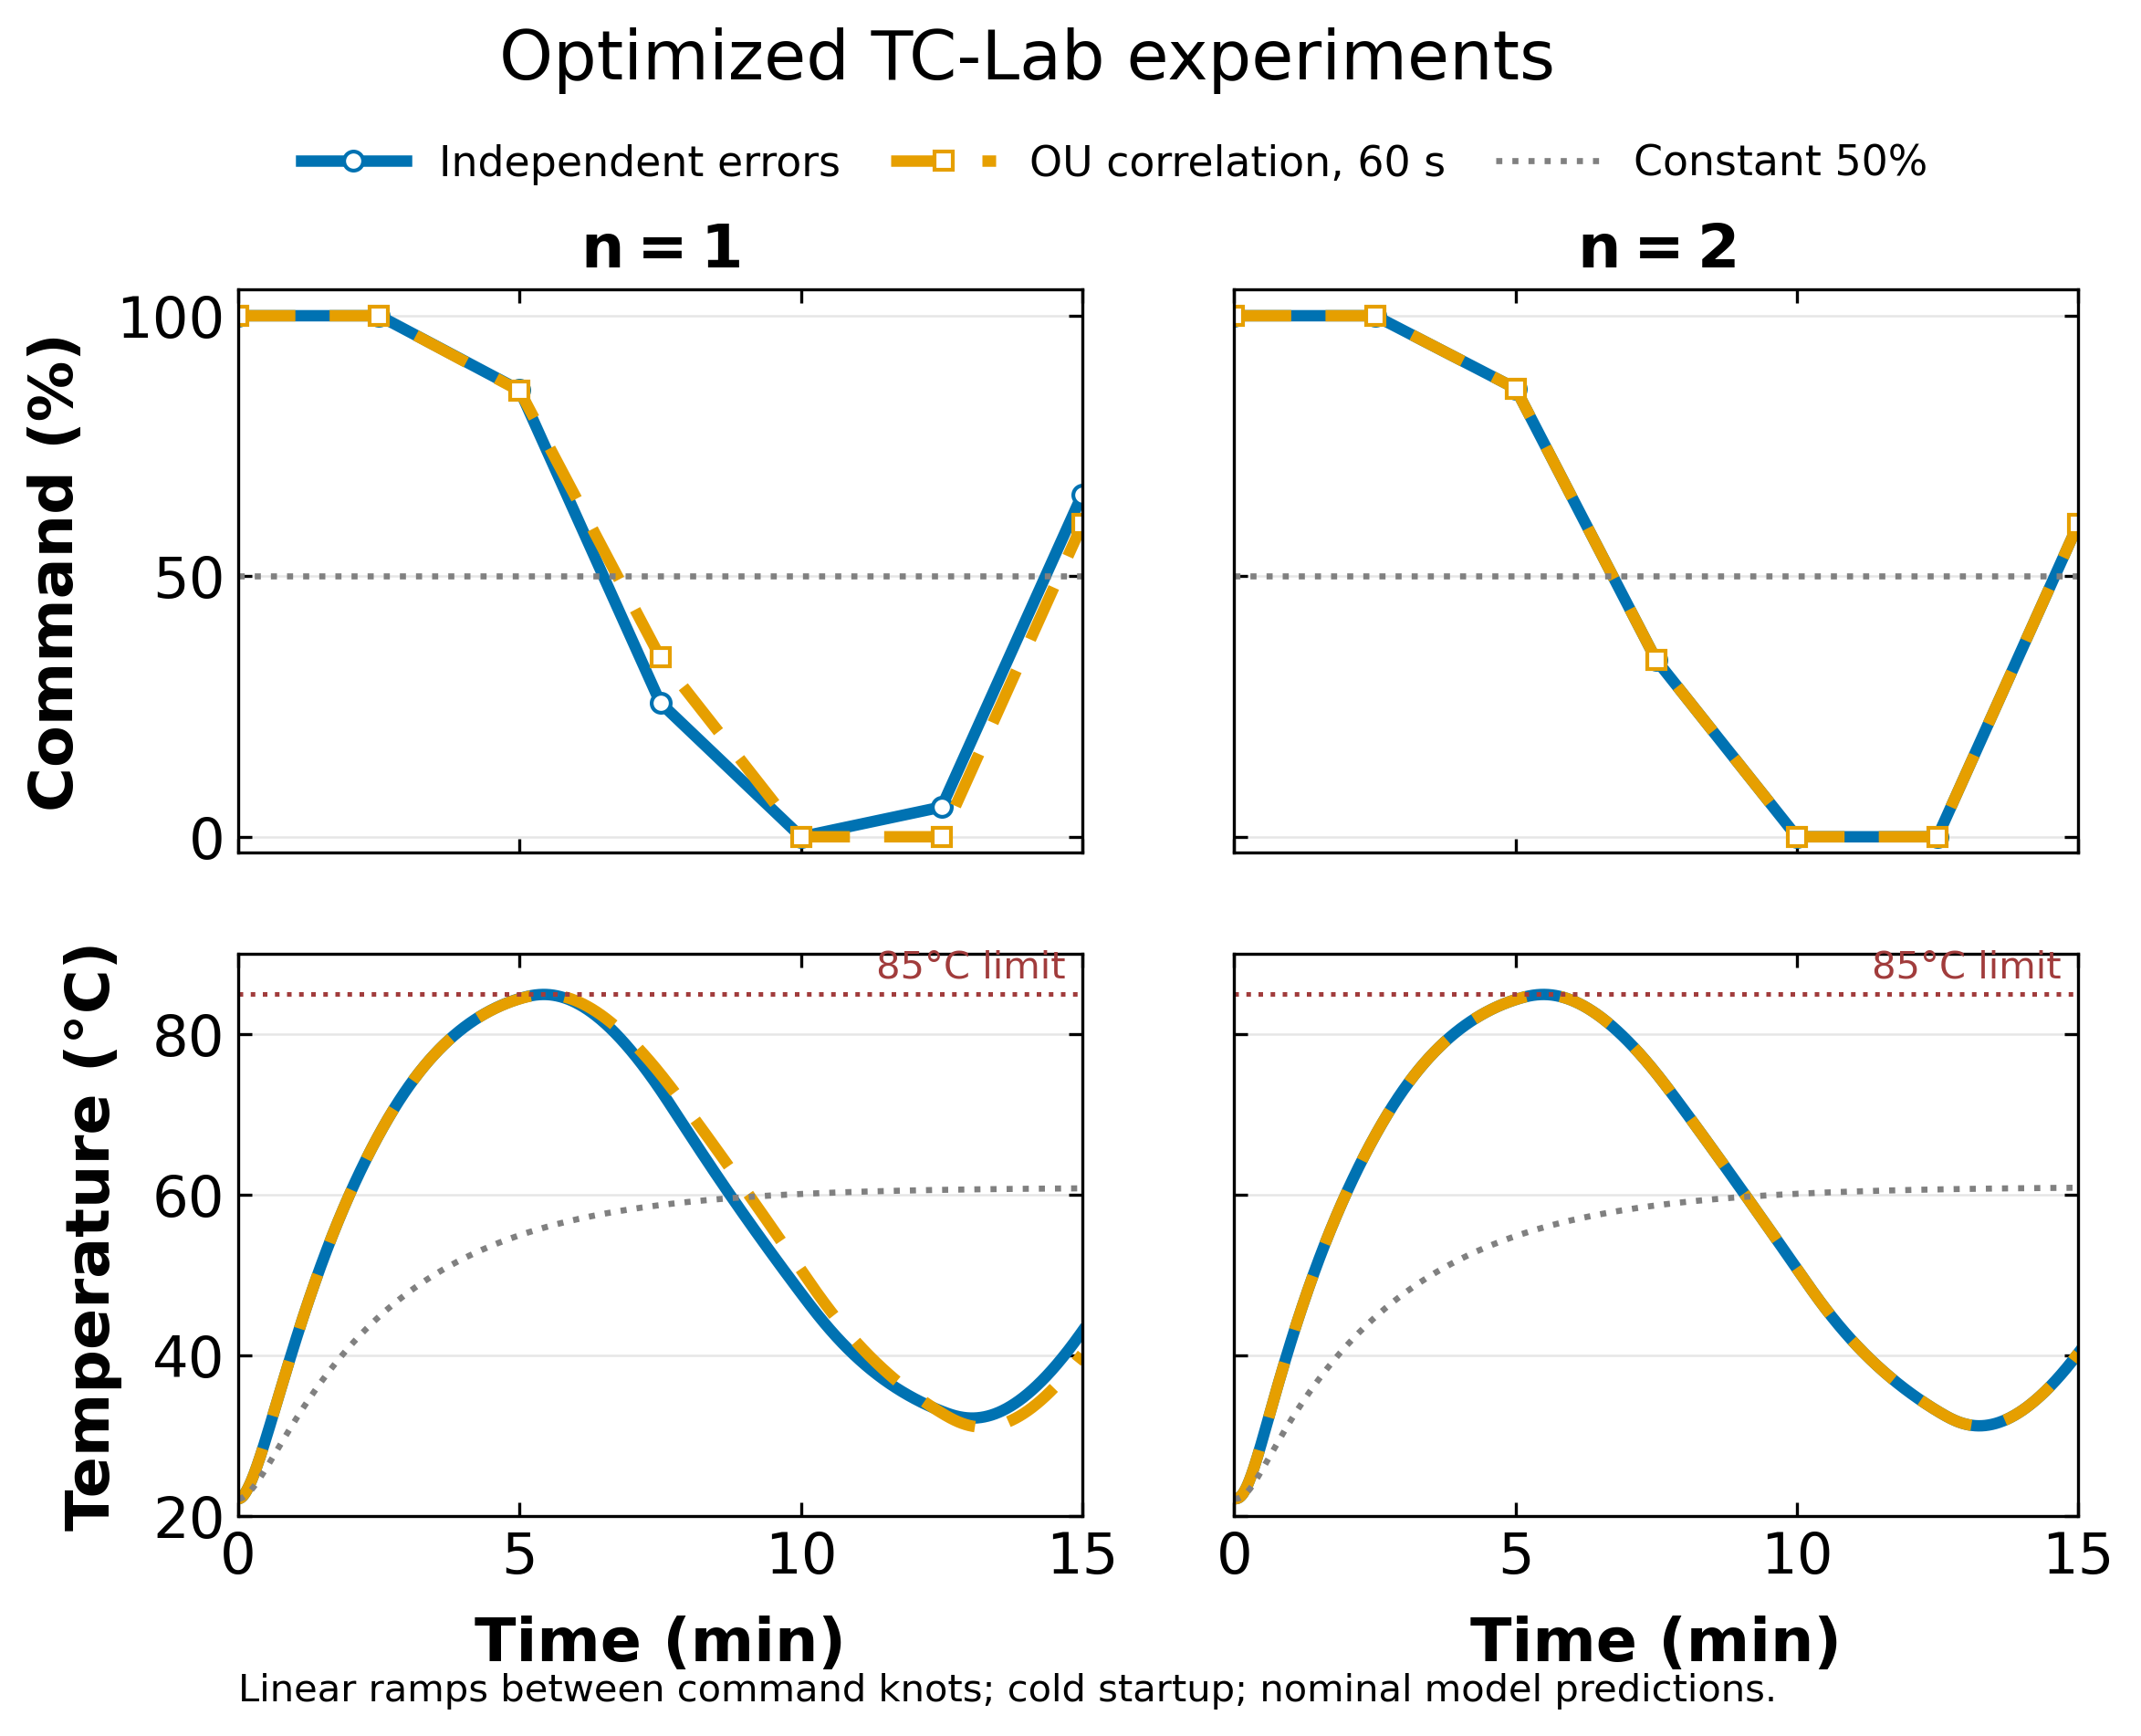
\includegraphics[width=\linewidth]{../teaching_followup/figures/optimized_experiments.png}
 \caption{Native Pyomo.DoE local D-optimal teaching experiments for three
 transfer parameters. Columns compare one and two delay stages. Upper panels
 show affine heater commands; lower panels show separately simulated nominal
 temperature responses on a $0.25$ s grid. Blue curves assume independent
 errors; orange curves assume known stationary OU correlation of $60$ s.
 Gray dotted curves use constant $50\%$ command with the same total dose.
 The red line is the imposed $85\,{}^\circ\mathrm C$ acceptance limit.
 Curves are conditional cold-start means; they are not uncertainty bands.}
 \label{fig:teaching-experiments}
\end{figure}
% Generated by teaching_followup/render_report_tables.py
\begin{table}[htbp]
\centering
\small
\caption{Selected heater command knots (percent), rounded to two decimals. Commands interpolate linearly; exact values are saved in the command CSV.}
\label{tab:teaching-commands}
\begin{tabular}{rrrrr}
\toprule
Time (min) & $n=1$ IID & $n=1$ OU60 & $n=2$ IID & $n=2$ OU60 \\
\midrule
0.0 & 100.00 & 100.00 & 100.00 & 100.00 \\
2.5 & 100.00 & 100.00 & 100.00 & 100.00 \\
5.0 & 85.71 & 85.60 & 86.06 & 86.06 \\
7.5 & 25.71 & 34.40 & 33.94 & 33.94 \\
10.0 & 0.00 & 0.00 & 0.00 & 0.00 \\
12.5 & 5.71 & 0.00 & 0.00 & 0.00 \\
15.0 & 65.71 & 60.00 & 60.00 & 60.00 \\
\bottomrule
\end{tabular}
\end{table}

\FloatBarrier

\subsection{Numerical checks and classroom scope}
An independent auditor checked all sixteen saved information matrices and local
SD evaluations: the baseline, two starts and a refined-mesh evaluation in each
case. It uses complex-step sensitivities from the study's exact simulator and
explicit full covariance inversion, independently of the Pyomo whitening
implementation. The largest relative FIM error is below $3.3\times10^{-7}$;
the largest relative local-SD error is below $2.6\times10^{-5}$.

Three-point Radau collocation uses $90$ finite elements for $n=1$ and $180$
for $n=2$, with the selected inputs also evaluated at twice those counts.
The initial $n=2$ mesh failed the $0.001\,{}^\circ\mathrm C$ mean tolerance
and was refined. An unnecessary lower bound on the collocation temperature
polynomial caused false infeasibility near startup; removing that bound
preserved the upper temperature constraint. Failed trials and the correction
to sensitivity evaluation at active design constraints are retained in
\path{teaching_followup/trial_failures.json}.

All four selected commands satisfy dose, amplitude and knot-change checks.
Their independently simulated temperatures remain below $85\,{}^\circ\mathrm C$
on the $0.25$ s grid over the proposed $900$ s window. This check covers the
nominal fitted points. Parameter uncertainty, continuous-time bounds, shutdown
after $900$ s and hardware operation require separate assessment.

For teaching, fit $n=1$, expose the original physical redundancy, compare
independent and correlated uncertainty, and optimize a varying input.
Use $n=2$ to ask whether an added delay stage changes prediction, global
identifiability or numerical requirements. The scripts, saved results,
independent audit and plotting receipt are under
\path{skunk_works/delay_study/teaching_followup}.
